\documentclass[]{article}
\usepackage{lmodern}
\usepackage{amssymb,amsmath}
\usepackage{ifxetex,ifluatex}
\usepackage{fixltx2e} % provides \textsubscript
\ifnum 0\ifxetex 1\fi\ifluatex 1\fi=0 % if pdftex
  \usepackage[T1]{fontenc}
  \usepackage[utf8]{inputenc}
\else % if luatex or xelatex
  \ifxetex
    \usepackage{mathspec}
  \else
    \usepackage{fontspec}
  \fi
  \defaultfontfeatures{Ligatures=TeX,Scale=MatchLowercase}
\fi
% use upquote if available, for straight quotes in verbatim environments
\IfFileExists{upquote.sty}{\usepackage{upquote}}{}
% use microtype if available
\IfFileExists{microtype.sty}{%
\usepackage{microtype}
\UseMicrotypeSet[protrusion]{basicmath} % disable protrusion for tt fonts
}{}
\usepackage[margin=1in]{geometry}
\usepackage{hyperref}
\hypersetup{unicode=true,
            pdftitle={The value of information for conservation auctions},
            pdfauthor={William K Morris},
            pdfborder={0 0 0},
            breaklinks=true}
\urlstyle{same}  % don't use monospace font for urls
\usepackage{natbib}
\bibliographystyle{voiConsAuc.bst}
\usepackage{longtable,booktabs}
\usepackage{graphicx,grffile}
\makeatletter
\def\maxwidth{\ifdim\Gin@nat@width>\linewidth\linewidth\else\Gin@nat@width\fi}
\def\maxheight{\ifdim\Gin@nat@height>\textheight\textheight\else\Gin@nat@height\fi}
\makeatother
% Scale images if necessary, so that they will not overflow the page
% margins by default, and it is still possible to overwrite the defaults
% using explicit options in \includegraphics[width, height, ...]{}
\setkeys{Gin}{width=\maxwidth,height=\maxheight,keepaspectratio}
\IfFileExists{parskip.sty}{%
\usepackage{parskip}
}{% else
\setlength{\parindent}{0pt}
\setlength{\parskip}{6pt plus 2pt minus 1pt}
}
\setlength{\emergencystretch}{3em}  % prevent overfull lines
\providecommand{\tightlist}{%
  \setlength{\itemsep}{0pt}\setlength{\parskip}{0pt}}
\setcounter{secnumdepth}{5}

%%% Use protect on footnotes to avoid problems with footnotes in titles
\let\rmarkdownfootnote\footnote%
\def\footnote{\protect\rmarkdownfootnote}

%%% Change title format to be more compact
\usepackage{titling}

% Create subtitle command for use in maketitle
\newcommand{\subtitle}[1]{
  \posttitle{
    \begin{center}\large#1\end{center}
    }
}

\setlength{\droptitle}{-2em}
  \title{The value of information for conservation auctions}
  \pretitle{\vspace{\droptitle}\centering\huge}
  \posttitle{\par}
  \author{William K Morris}
  \preauthor{\centering\large\emph}
  \postauthor{\par}
  \predate{\centering\large\emph}
  \postdate{\par}
  \date{2017-09-05}

\usepackage{titlesec}
\titleformat{\paragraph}{\small\normalfont\bfseries}{}{0pt}{}
\titleformat{\subparagraph}{\small\normalfont}{}{0pt}{}
\linespread{2}\selectfont
\usepackage{booktabs}
\usepackage{setspace}
\usepackage{caption}
\usepackage{tikz}
\usepackage{pdflscape}
\captionsetup{font={stretch=2}}
\usepackage{pbox}
\usepackage[displaymath,mathlines]{lineno}
\linenumbers

\usepackage{amsthm}
\newtheorem{theorem}{Theorem}[section]
\newtheorem{lemma}{Lemma}[section]
\theoremstyle{definition}
\newtheorem{definition}{Definition}[section]
\newtheorem{corollary}{Corollary}[section]
\newtheorem{proposition}{Proposition}[section]
\theoremstyle{definition}
\newtheorem{example}{Example}[section]
\theoremstyle{remark}
\newtheorem*{remark}{Remark}
\begin{document}
\maketitle


\subsection*{Abstract}\label{abstract}
\addcontentsline{toc}{subsection}{Abstract}

Conservation auctions are tools for natural resource managers to cost-efficiently protect biodiversity and ecosystem services. Benefits particularly induce uncertainty in the value to be maximised. Therefore learning about benefits is valuable to decide which bids will be successful. Here we use the concept of expected value of sample information to assess how an agency should allocate a limited learning budget among bids to conduct a conservation auction that yields the most cost-efficient return on investment. We propose a simple model where an agent has two or more assets among which they must pick the single most cost-efficient to invest in with an auction. The cost-efficiency of each asset is more or less uncertain and there is some budget allocated to reduce the uncertainty of the assets. The agent must decide how to allocate the learning budget among the assets to maximize the expected benefit of the auction. Using a mix of analytical, heuristic and simulation solutions to the model we glean a number of rules-of-thumb that may be helpful to agencies conducting conservation auctions. When learning budgets are small, then it is best to learn about the most marginal assets. Then, as the budget increases it becomes more optimal to learn about assets which have uncertain cost-efficiency in the more general sense. Finally, as learning budgets become large enough, resources can be allocated evenly across all uncertain assets. Our findings imply that a naive even allocation to learning among assets in a conservation auction may lead to less than cost-efficient outcomes.

\subsection*{Introduction}\label{introduction}
\addcontentsline{toc}{subsection}{Introduction}

Conservation auctions have become a widespread and established market
mechanism aimed at achieving public environmental good by contracting
with landholders and managers cost-efficiently \citep{Schomers2013}.
Conservation auctions include payment for ecosystem services (PES)
schemes \citep{Engel2008}, environmental stewardship \citep{Ribaudo2008}
and conservation easement programs \citep{Brown2011}. Some recent
examples include the US Water Quality Incentives Program
\citep{Kraft1996}, the English Countryside Stewardship Scheme
\citep{Lobley1998}, and Bush Tender in Victoria, Australia
\citep{Stoneham2003}.

Uncertainty about the benefits resulting from a conservation auction
investment is not often addressed. For example, in implementing a
conservation auction to facilitate vegetation regeneration, the
Goulburn-Broken Catchment Management Authority \citep{Miles2008} used
what they call a restoration benefit index (RBI) to rank auction bids.
While the RBI included multiple components, including conservation
significance, regeneration potential and landholder management action,
it did not include any measure of uncertainty. Ignoring uncertainty, one
may forego untapped benefit in the implementation of a conservation
auction. If the uncertainty in a conservation auction was first
characterized and then reduced, then it could potentially be implemented
more cost-efficiently, because one could better identify the superior
conservation assets.

Here we consider learning to reduce uncertainty in a conservation
auction and how resources should be allocated among the assets available
for investment. We use the concept of expected value of sample
information (EVSI) \citep{Raiffa1961} and a simple auction model to
discover the best strategy to allocate resources to learning in a
conservation auction. With our model and the solutions we provide below,
we derive three guiding principles that will aid an agency undertaking a
conservation auction in allocating resources to learning about the
cost-efficiency of the assets in their auction pool. The rest of the
manuscript is structured as follows: first we describe in more detail
how conservation auctions work and then briefly introduce the reader to
theory of expected value of sample information. We then formalise a
problem of information valuing for conservation auctions, describing how
uncertainty is pertinent in this context. We then demonstrate our
solutions to the problem presented before finally summarizing the
findings with a set of principles that practitioners should heed when
implementing a conservation auction with uncertain benefits. We have
kept our final discussion brief as in opening up a diversity of fronts
for thinking about learning for conservation auctions, this work is
necessarily preliminary and exploratory.

\subsubsection*{Reverse auctions}\label{reverse-auctions}
\addcontentsline{toc}{subsubsection}{Reverse auctions}

Conservation auctions often take the form of a reverse auction
\citep[though sometimes conservation auctions are standard auctions see
e.g.,][]{Toth2013}. In a reverse auction, the agency conducting the
auction, usually a branch of a government, is the buyer. The bidders are
the landholders or land-managers who compete for the pool of funding
available by offering to sell some prespecified environmental good
desired by the auction-conducting agency \citep{Mcafee1987}. The
environmental good may take the form of land title or a contract to
conduct particular management actions. In some cases the outcome of
management is the good specified in the contract and the management
action is left up to the managers \citep{Hanley2014}. Unlike a standard
auction where the buyers are competing and price is maximized, reverse
auctions are aimed at reducing the price of the goods being purchased,
as it is the sellers who are in competition with one another. In
facilitating the competition for a single pool of funding, the auction
conducting agent seeks to maximize the environmental benefit it can get
for the lowest cost and thus maximize the cost-efficiency of the
environmental scheme \citep{Latacz1997}.

\subsubsection*{Ranking auction bids by
cost-efficiency}\label{ranking-auction-bids-by-cost-efficiency}
\addcontentsline{toc}{subsubsection}{Ranking auction bids by
cost-efficiency}

In a typical reverse auction, aimed at getting some public environmental
good, the conducting agency will assess the bids by their
cost-efficiency. The bids will be ranked from highest to lowest in terms
of cost-efficiency \citep{Stoneham2003}. The winning bids will be the
most cost-efficient down to some cutoff. The cutoff may be the
cumulative total cost of the most cost efficient bids measured against a
fixed budget, or it could be a prespecified level of cost-efficiency
\citep{Latacz1997}. Time-limited reverse auctions will often use the
budget exhaustion method whereas longer-term schemes with repeated
rounds might use a cost-efficiency-based cutoff. The
rank-by-cost-efficiency strategy is usually near optimal, though in some
circumstances it can produce non-optimal results and more sophisticated
portfolio methods can be used to maximize the total benefit. When there
are many cheap assets in the auction pool the method tends to work well,
but in cases where the bids consist of a small number of expensive
assets, overall performance may be reduced considerably
\citep{Hajkowicz2007}.

\subsubsection*{Conservation auctions and
uncertainty}\label{conservation-auctions-and-uncertainty}
\addcontentsline{toc}{subsubsection}{Conservation auctions and
uncertainty}

There are multiple sources of uncertainty in a conservation auction that
can affect the outcome in a number of ways. Moreover, there are multiple
perspectives from which to view uncertainty within the framework of a
conservation auction, and the different actors may be affected by
different uncertainties about different aspects of the auction. Here we
focus only one aspect of uncertainty: uncertainty about the
cost-efficiency of bids and only from the perspective of the agency
conducting the auction. Other important facets of uncertainty in
reverse-auctions, are the knowledge bidders have of one another's
circumstances and intentions, and the circumstances of the seller. There
is a vast game-theoretic literature dealing with these types of
uncertainty in auctions \citep[see for example][]{Hailu2004}, but we
don't deal with them further here.

After the bids are submitted in an auction, that component of the
auction cost will have no uncertainty. So in most conservation auctions
the bulk of the uncertainty about cost-efficiency is due to uncertainty
about benefits. Conservation benefit of the kind sought after in a
reverse auction is inherently uncertain, as it is often only realized at
some point far in future, long after the auction scheme is implemented.
Land regeneration, water or soil quality improvement, or other ecosystem
services are some examples of the type of benefit that is paid for at
one point in time, while the payoff is not expected until much later on
\citep{Vesk2008}. This time-lag in return on investment is one issue
that makes the cost-efficiency of auction bids uncertain. Uncertainty in
the individual auction bids then leads to a necessary uncertainty in
their ranking. And therefore, the uncertainty in benefits flows through
to the cost-efficiency and to the total benefit realized for the
conservation auction scheme.

\subsubsection*{The value of
information}\label{the-value-of-information}
\addcontentsline{toc}{subsubsection}{The value of information}

Given that the outcome of many conservation auctions maybe uncertain, it
may be wise for an auction conducting agency to invest resources in
learning about the benefits before they rank the assets and determine
the winning bids. If they can increase the probability of correctly
ranking the bids in order of cost-efficiency, they could avoid investing
in unwarranted assets and increase the total benefits realized after the
auction is completed. The performance gain one might expect after
learning and a subsequent reduction in uncertainty is known as the
expected value of information (EVI) \citep{Raiffa1961}. Decision makers
can use an EVI analysis to predetermine the worth of learning about the
outcome a decision problem such as a conservation auction. A type of EVI
is the expected value of sample information (EVSI), which is the value
of reducing uncertainty by some degree, by collecting a sample of data,
as opposed to eliminating uncertainty completely, which is the expected
value of perfect information (EVPI) \citep{Yokota2004b}.

Using the concept of EVSI, a conservation auctioneer could work out if
it would be worthwhile collecting data to learn about the benefits of a
conservation auction and even how much data would be most to appropriate
to collect. Here we extend the idea of expected value of sample
information for a conservation auction and consider how to allocate the
learning effort among the different assets available in the auction. The
naive solution to problem is simply to allocate learning evenly among
the assets and reducing the uncertainty about the benefits of each by
the same degree. However, depending on the particular circumstances of
the initial levels of uncertainty, this may not be the most optimal
allocation of learning resources.

\subsection*{Analysis}\label{analysis}
\addcontentsline{toc}{subsection}{Analysis}

\subsubsection*{The Model}\label{the-model}
\addcontentsline{toc}{subsubsection}{The Model}

Here we describe a simple model of a conservation auction where the
cost-efficiency of each asset in the auction pool is uncertain. In our
model, there are \(n>1\), assets. The \(i^{th}\) (\(i = 1...n\))
asset's, \(A_i\), cost-efficiency, \(c_i\), is described by a normal
distribution with mean, \(\mu_i\) and standard deviation, \(\sigma_i\).
There are two separate budgets, one for investing in assets in the
reverse auction and a second budget that can be used to reduce the
uncertainty about the assets' cost-efficiencies. The first budget is
large enough to invest in any one of the assets, while the second budget
is variable and can be used to collect a sample of data about the
cost-efficiency of each individual asset. In the hypothetical case we
consider here, the agency has an oppurtunity to collect new information
after bids are made but before the successful bids are decided. The
total budget for data collection \(M\), may be divided between each of
the \(n\) assets in the auction with a different proportion, \(p_i\),
allocated to each asset, where \(Mp_i\) is proportional to the
sample-size of data collected about the cost-efficiency of the
\(i^{th}\) asset. Here, \(M\) can be considered to be the total
sample-size assuming that the sampling variance is one. An increase in
sample-size or reduction in sampling variance would both increase the
effective budget size.

\subsubsection*{Expected value under
uncertainty}\label{expected-value-under-uncertainty}
\addcontentsline{toc}{subsubsection}{Expected value under uncertainty}

Under the initial uncertainty, a risk-neutral auctioneer would simply
rank the assets in order of their expected cost-efficiency and invest in
the asset with the highest expected cost-efficiency. This is the
expected value under uncertainty or also known as the expected value
with original information (EVWOI). More formally,

\begin{equation}
\mathrm{EVWOI} = \max_i(\mu_i)
\label{eq:EVWOIan}
\end{equation}

\subsubsection*{Expected value of sample
information}\label{expected-value-of-sample-information}
\addcontentsline{toc}{subsubsection}{Expected value of sample
information}

Now we turn to the allocation of sampling among the assets in the
auction pool and the calculation of the EVSI. In the following sections
we outline three solutions to the problem of calculating EVSI for the
model above, given a sampling budget and an allocation of the budget
among the assets in the auction pool. The first is an analytical
solution which applies when \(n = 2\). For \(n = 3\), the analytical
solution does not apply, so we have formulated a heuristic definition.
The heuristic definition of EVSI is based on valuing the rank order of
cost-efficiency rather than actual benefit achieved. We then compare
these solutions to a general solution using Monte Carlo simulation. All
analysis has been implemented in the programming language R
\citep{R2017} unless otherwise stated.

\paragraph*{\texorpdfstring{Analytical solution for
\(n = 2\)}{Analytical solution for n = 2}}\label{analytical-solution-for-n-2}
\addcontentsline{toc}{paragraph}{Analytical solution for \(n = 2\)}

When \(n = 2\) an analytical solution exists. Its derivation can be
found in \citet{Moore2017} where EVSI is defined as:

\begin{equation}
\mathrm{EVSI} = \frac{1}{2}\left(\Theta\sqrt{\frac{2}{\pi}}e^{-\frac{\mu_1 - \mu_2}{2\Theta^2}} + (\mu_1 - \mu_2)\,\mathrm{erf}\left(\frac{\mu_1 - \mu_2}{\Theta\sqrt{2}}\right) - |\mu_1 - \mu_2|\right)
\label{eq:evsi2anp1}
\end{equation}

\clearpage

where,

\begin{equation}
\Theta = \sqrt{\sigma^2_1\frac{Mp_1\sigma^2_1}{Mp_1\sigma^2_1 + 1} + \sigma^2_2\frac{Mp_2\sigma^2_2}{Mp_2\sigma^2_2 + 1}}
\label{eq:evsi2anp2}
\end{equation}

Note that to calculate the EVPI one can replace equation
\eqref{eq:evsi2anp2} with \(\Theta = \sqrt{\sigma^2_1 + \sigma^2_2}\).
With the above definition we can find the value of \(p_1\) (where
\(p_2 = 1 - p_1\)) that maximizes EVSI for a given budget, \(M\). To
find the optimal solutions we used a combination of golden section
search and successive parabolic interpolation \citep[as implemented
in][]{Forsythe1977}.

In figure \ref{fig:evsi2anplot} we show the results of such an
optimization for a case where one asset has high expected
cost-efficiency and high uncertainty and the other asset has relatively
lower expected cost-efficiency and uncertainty. Using a heuristic
solution (discussed below and in Appendix C) we arrive at exactly the
same solution.

In examining either the analytic or heuristic solutions for \(n = 2\),
we find that when the assets have different amounts of uncertainty about
their respective cost-efficiencies the optimal strategy is to learn only
about the more uncertain asset when the budget is low. Then, if the
budget is increased, allocation to learning can gradually switch to
learning about both assets. When the budget is sufficiently large, then
learning can be allocated evenly between the assets. Figure
\ref{fig:evsi2anplot2} shows how this allocation depends on the ratio of
\(\sigma_1\) and \(\sigma_2\) for a fixed ratio means. The ratio of the
means though, does not affect the optimal allocation (Appendix C).
















\begin{figure}[htbp]
\centering
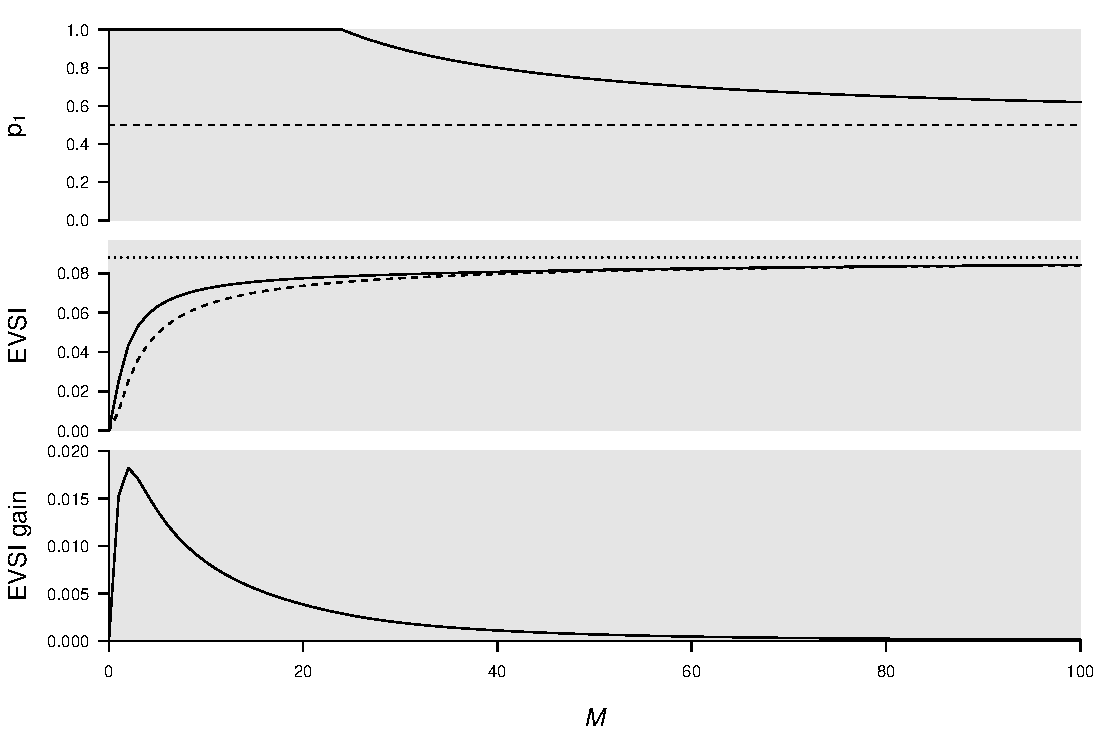
\includegraphics{voiConsAuc_files/figure-latex/evsi2anplot-1.pdf}
\caption{\label{fig:evsi2anplot}Analytical solution to optimal allocation of sampling
between two assets. In this case, the two assets have prior
distributions \(\mathrm{N}(1,1)\) and \(\mathrm{N}(0,0.2)\)
respectively. The top panel indicates the optimal proportional
allocation of sampling between the two assets (solid line) as well as
the naive allocation with even sampling between two assets (dashed
line). Here \(p_1\) is the proportion allocated to the first asset and
\(M\) is the total number of samples (the budget). The middle panel
shows the EVSI for the optimal and naive sampling strategies of the
panel above. The dotted line is the EVPI (0.09). The solid line
indicates the EVSI for the optimal allocation while the dashed line is
the naive allocation. The bottom panel indicates the gain in EVSI of
using the optimal strategy over the naive solution (the difference
between the two curves in the middle panel).}
\end{figure}






\begin{figure}[htbp]
\centering
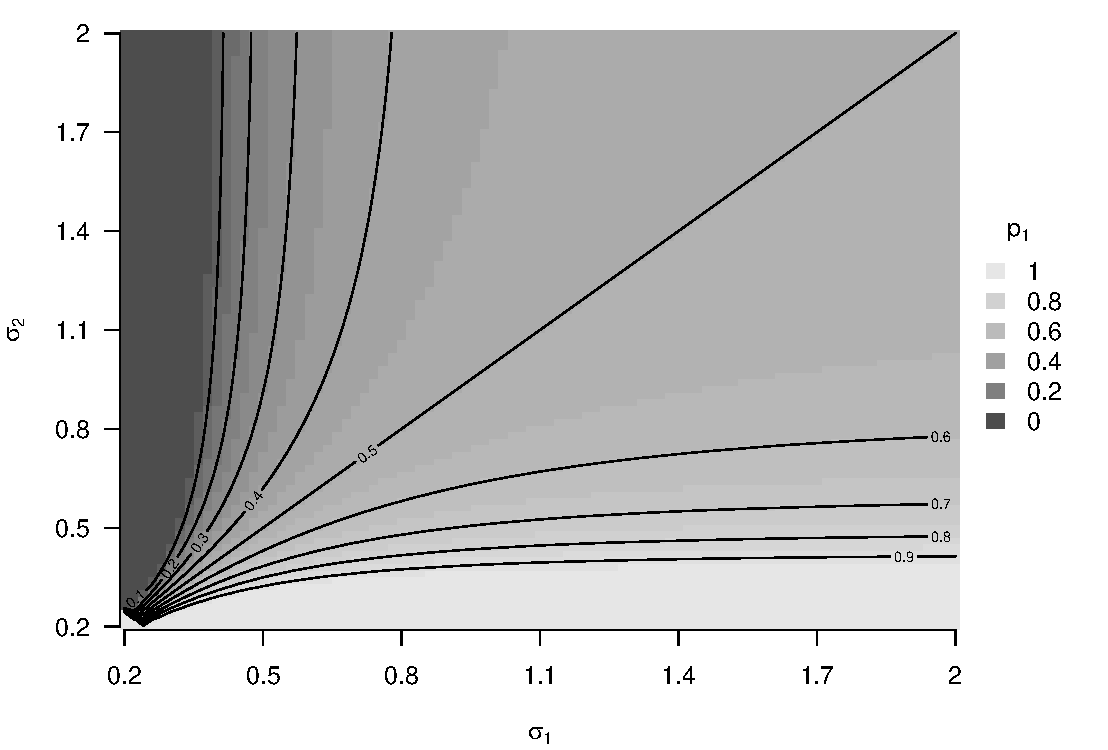
\includegraphics{voiConsAuc_files/figure-latex/evsi2anplot2-1.pdf}
\caption{\label{fig:evsi2anplot2}Relationship between optimal allocation to asset 1,
\(p_1\), and the parameters \(\sigma_1\) and \(\sigma_2\), according to
both the analytical and heuristic solutions. Here \(M=7\), \(\mu_1=1\)
and \(\mu_2=0\).}
\end{figure}

\clearpage

\paragraph*{\texorpdfstring{Heuristic solution for
\(n = 3\)}{Heuristic solution for n = 3}}\label{heuristic-solution-for-n-3}
\addcontentsline{toc}{paragraph}{Heuristic solution for \(n = 3\)}

As the analytical solution above does not hold for \(n > 2\) we propose
the following heuristic solution (when applied to \(n = 2\) the
heuristic solution allocates learning in exactly the same manner as the
analytical solution, see Appendix C) based on valuing the rank order of
cost-efficiency of assets in the auction pool. To elaborate, in valuing
the assets by rank, we mean we assign utilities to choosing a single
asset that is ranked first, second or third in terms of cost-efficiency.
In this sense, utility is indifferent to how much better, for example,
the first-ranked asset is than the second and only concerned that it is
the better of the two assets. With this principle we assign utilities,
\(u\), to each combination of asset choice, \(A_i\), and true rank order
of \(c_i\) such that:

\begin{equation}
\begin{aligned}
u(A_1, c_1 > c_2 > c_3)&=1\\
u(A_1, c_1 > c_3 > c_2)&=1\\
u(A_1, c_2 > c_1 > c_3)&=0.5\\
u(A_1, c_3 > c_1 > c_2)&=0.5\\
u(A_1, c_2 > c_3 > c_1)&=0\\
u(A_1, c_3 > c_2 > c_1)&=0\\
u(A_2, c_2 > c_1 > c_3)&=1\\
\mathrm{etc...}&
\end{aligned}
\label{eq:utilities}
\end{equation}

So here, one receives utility 1 when the chosen asset is truly top
ranked, but only utility 0.5 when the chosen asset is in fact the second
ranked. Note that the choice of utilities is arbitrary and that a
different set of values will change the solution. However, as long as
the order of the utilities is the same, the general shape of the
solution remains. It is this that makes the solution heuristic rather
than exact.

To determine EVSI given the above utilities we need only determine the
probability of each rank order and calculate the expected utility of
choosing each action with either the original or updated knowledge of
the asset cost-efficiencies.

We can express the probability of the assets being in a given rank order
as the probability of two differences being less than zero. Such that,
for example,

\begin{equation}
\Pr(c_1 > c_2 > c_3) = \Pr(c_2 - c_1 < 0,  c_3 - c_2 < 0)
\label{eq:probrank}
\end{equation}

Following this we define two new variables, \(z_1\) and \(z_2\) where

\begin{equation}
\begin{aligned}
  z_1 &= c_2 - c_1,\\
  z_2 &= c_3 - c_2
\end{aligned}
\label{eq:z12}
\end{equation}

When \(c_i\) are uncorrelated then the covariance of \(z_1\) and \(z_2\)
is \(-\sigma^2_2\) and they will have a joint distribution defined as:

\begin{equation}
\begin{bmatrix}z_1\\z_2\end{bmatrix}
  \sim\mathrm{N}\left(
  \begin{bmatrix}\mu_2-\mu_1\\\mu_3-\mu_2\end{bmatrix},
  \begin{bmatrix}\sigma^2_1+\sigma^2_2&-\sigma^2_2\\-\sigma^2_2&\sigma^2_2+\sigma^2_3\end{bmatrix}\right)
\label{eq:jointz}
\end{equation}

Given this joint distribution we can calculate \(\Pr(c_1 > c_2 > c_3)\)
by evaluating the multivariate normal cumulative distribution function,
\(\Phi(z_1, z_2)\) within the limits, \(-\infty\) and \(0\), using the
algorithm of Genz \citeyearpar{Genz1992}.

With the above, we can calculate the EVWOI, which is the maximum of the
expected utilities of choosing the \(i^{th}\) asset:

\begin{equation}
\mathrm{EVWOI} = \mathrm{max}(\mathrm{E}[u(A_i)])
\label{eq:EVWOIheu}
\end{equation}

where each expected value is the sum of the utilities assigned for that
choice of asset, multiplied by the rank order probabilities defined
above. For example,

\begin{equation}
\begin{aligned}
  \mathrm{E}[u(A_1)] = & 1 \times \Pr(c_1 > c_2 > c_3) + 1 \times \Pr(c_1 > c_3 > c_2)\,+ \\
  &0.5 \times \Pr(c_2 > c_1 > c_3) + 0.5 \times \Pr(c_3 > c_1 > c_2)\,+ \\
  &0 \times \Pr(c_2 > c_3 > c_1) + 0 \times \Pr(c_3 > c_2 > c_1)
\end{aligned}
\label{eq:EuA1}
\end{equation}

To calculate the EVSI we need not only know the EVWOI, but also the
expected value with sample information (EVWSI), for EVSI is the
magnitude of their difference:

\begin{equation}
\mathrm{EVSI} = \mathrm{max}(\mathrm{E}[u(A^\prime_i)]) - \mathrm{max}(\mathrm{E}[u(A_i)])
\label{eq:EVSIheu}
\end{equation}

Where EVWOI relied on the expected utilities under the prior knowledge
of cost efficiency ranking, the EVWSI relies on the expected utility
under the posterior (after knowledge of cost efficiency ranking has been
improved). To go from the expected utility under the prior,
\(\mathrm{E}[u(A_i)]\), to expected utility under the posterior,
\(\mathrm{E}[u(A^\prime_i)]\), we need to adjust the variances in
equation \eqref{eq:jointz} from \(\sigma^2_i\) to
\(\sigma^{\prime{}2}_i\), where

\begin{equation}
\sigma^{\prime{}2}_i = \frac{\sigma^2_i}{Mp_i\sigma^2_i + 1}
\label{eq:updatesigma}
\end{equation}

which accounts for the new information given the sampling allocation
\(Mp_i\).

With equation \eqref{eq:updatesigma}, we can find the optimal values of
\(p_i\) for any given learning budget, \(M\), and set of prior
distributions describing uncertainty in cost-efficiency, \(c_i\). To
find the optimal allocation of \(M\) we performed a constrained
optimization using the algorithm of Nelder and Mead
\citeyearpar{Nelder1965}. Figure \ref{fig:evsi3heuplot} shows such an
optimal allocation of \(M\) for a case where the expected
cost-efficiency and level of uncertainty varies across the three assets.
Appendix D contains an examination of the optimal allocation of learning
to three assets over increasing \(M\) and for different combinations of
uncertainty in the three asset's cost-efficiencies of which figure
\ref{fig:evsi3heuplot} is one example.

The important difference between the \(n=3\) cases and the simpler
version where \(n=2\) is that adding another asset now means that having
a heterogeniety prior means now has an effect on optimal allocation.
Where before (\(n=2\)), having different means, but the same degree of
unceratinty across assets, meant that the optimal allocation was always
to allocate learning evenly, when \(n=3\) in a case with equal
uncertainty across assets, different prior means alone will lead to a
uneven optimal allocation of learning (see e.g.~Appendix D, case-study
2b). Here we summarise the findings of the case-studies in Appendix C
and D with set of principles that may be applied to a conservation
auction during a pre-auction learning phase (see section: principles for
allocating resources to learning).









\begin{figure}[htbp]
\centering
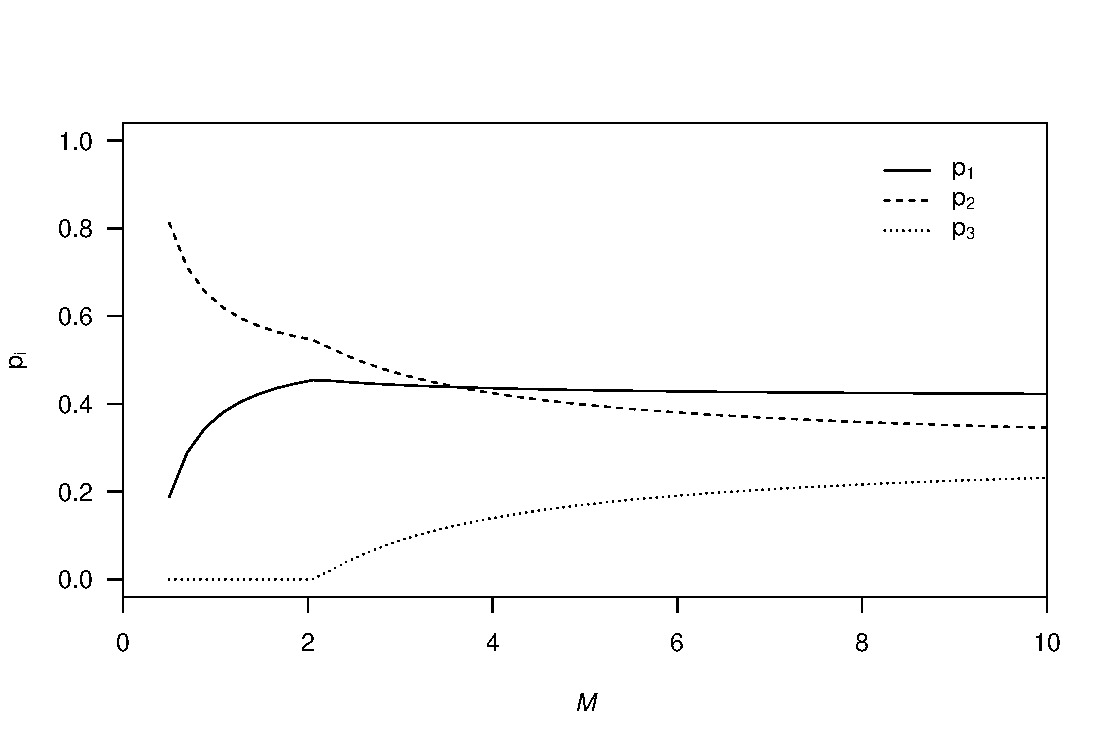
\includegraphics{voiConsAuc_files/figure-latex/evsi3heuplot-1.pdf}
\caption{\label{fig:evsi3heuplot}Heuristic solution to the optimal allocation of
sampling among three assets. In this case the assets have prior
distributions of \(N(1, 0.8)\), \(N(0.5, 1.25)\) and \(N(0.5, 0.75)\)
describing the uncertainty in the cost-efficiency respectively. The
curves show the optimal allocation, \(p_i\), of the sampling budget,
\(M\), to the first (solid line), second (dashed line) and third (dotted
line) assets.}
\end{figure}

\paragraph*{Monte Carlo Simulation}\label{monte-carlo-simulation}
\addcontentsline{toc}{paragraph}{Monte Carlo Simulation}

Finally we present a general solution to calculate the EVSI for the
model with Monte Carlo simulation. The simulation uses an algorithm we
have implemented in the programming language Julia \citep{Bezanson2017}
and presented in the pseudo code below.

\begin{center}\rule{0.5\linewidth}{\linethickness}\end{center}

\textbf{Begin outer loop}: for \(s\) of 1 to \(S\) simulations

\textbf{Begin inner loop}: for \(i\) of 1 to \(n\) assets

\begin{enumerate}
\def\labelenumi{\arabic{enumi}.}
\item
  Draw a \emph{true} value, \(c^*_{s,i}\), at random from prior
  distribution \(\mathrm{N}(\mu_i, \sigma_i)\)
\item
  Draw a sample mean, \(y_{s,i}\), at random from
  \(\mathrm{N}(c^*_{s, i}, \sqrt{\frac{1}{Mp_i}})\)
\item
  Calculate a posterior mean \(\mu^\prime_i\) as weighted sum of prior
  and sample means
  \(\mu_i \frac{\frac{1}{\sigma_i}}{Mp_i + \frac{1}{\sigma_i}} + y_{s,i}\frac{Mp_i}{Mp_i + \frac{1}{\sigma_i}}\)
\end{enumerate}

\textbf{End inner loop}

\begin{enumerate}
\def\labelenumi{\arabic{enumi}.}
\setcounter{enumi}{3}
\tightlist
\item
  Calculate value given sample information, \(v_s\), as \emph{true}
  value of asset with largest posterior mean
  \(c^*_{s,\mathrm{argmax}_i(\mu^\prime_i)}\)
\end{enumerate}

\textbf{End outer loop}

\begin{enumerate}
\def\labelenumi{\arabic{enumi}.}
\setcounter{enumi}{4}
\tightlist
\item
  Calculate \(\mathrm{EVSI}\) as expected value given sample
  information, \(\frac{1}{S}\sum\limits_{s = 1}^{S} v_s\), minus
  expected value given prior information, \(\max_i({\mu_i})\)
\end{enumerate}

\begin{center}\rule{0.5\linewidth}{\linethickness}\end{center}

While the algorithm is relatively simple to implement and gives unbiased
estimates of EVSI, it is computationally expensive and the estimates are
relatively imprecise. Moreover the impact of this imprecision increases
with \(M\), as changes in EVSI in response to changes in \(p_i\) are
more subtle for larger budgets. Therefore, we use the simulation as a
tool to validate assertions about optimal allocation of learning
resources based on the heuristic solutions above. Figures
\ref{fig:evsi2simplot} and \ref{fig:evsi3simplot} illustrate the
application of the simulation solution to the same case studies outlined
in figures \ref{fig:evsi2anplot} and \ref{fig:evsi3heuplot}
respectively.










\begin{figure}[htbp]
\centering
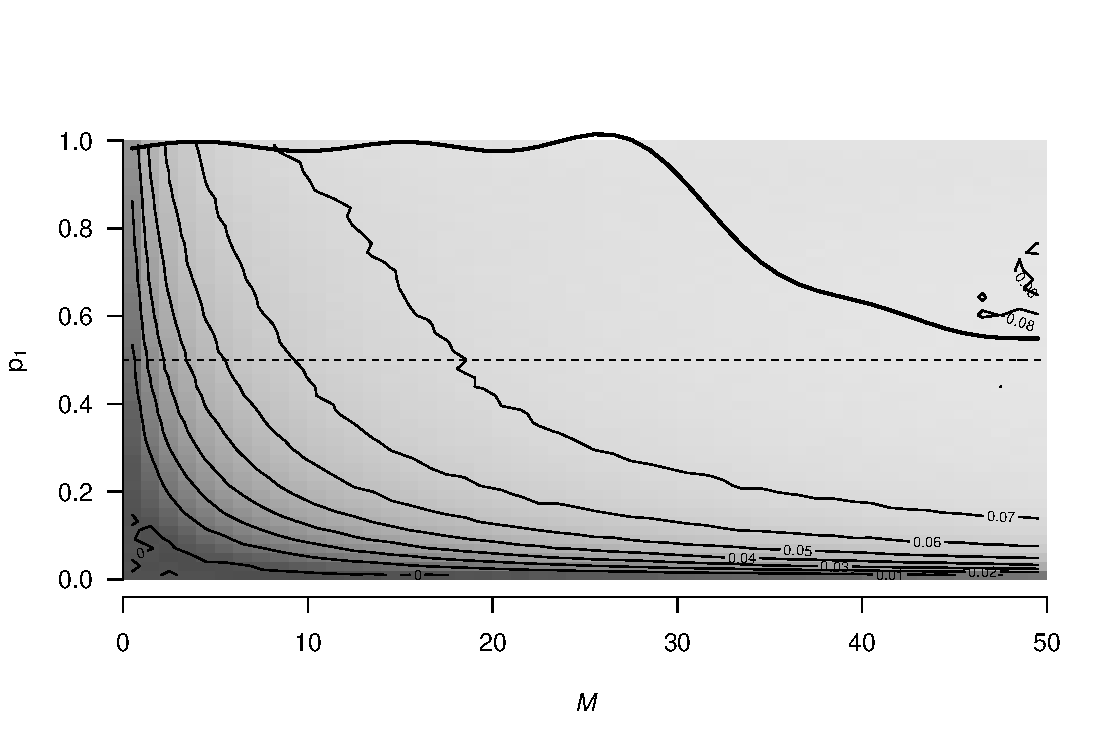
\includegraphics{voiConsAuc_files/figure-latex/evsi2simplot-1.pdf}
\caption{\label{fig:evsi2simplot}Simulation of EVSI for different allocations of
sampling effort among two assets with increasing budget. Again, the two
assets have prior distributions \(\mathrm{N}(1,1)\) and
\(\mathrm{N}(0,0.2)\) respectively. Contours and shading indicates the
estimated EVSI for the given allocation and budget. Solid line is a
smoothed curve fit to the optimal (maximum EVSI) value of \(p_1\) for
each budget. Note that this curve has a similar shape to analytical
solution in the top panel of figure \ref{fig:evsi2anplot}.}
\end{figure}








\begin{figure}[htbp]
\centering
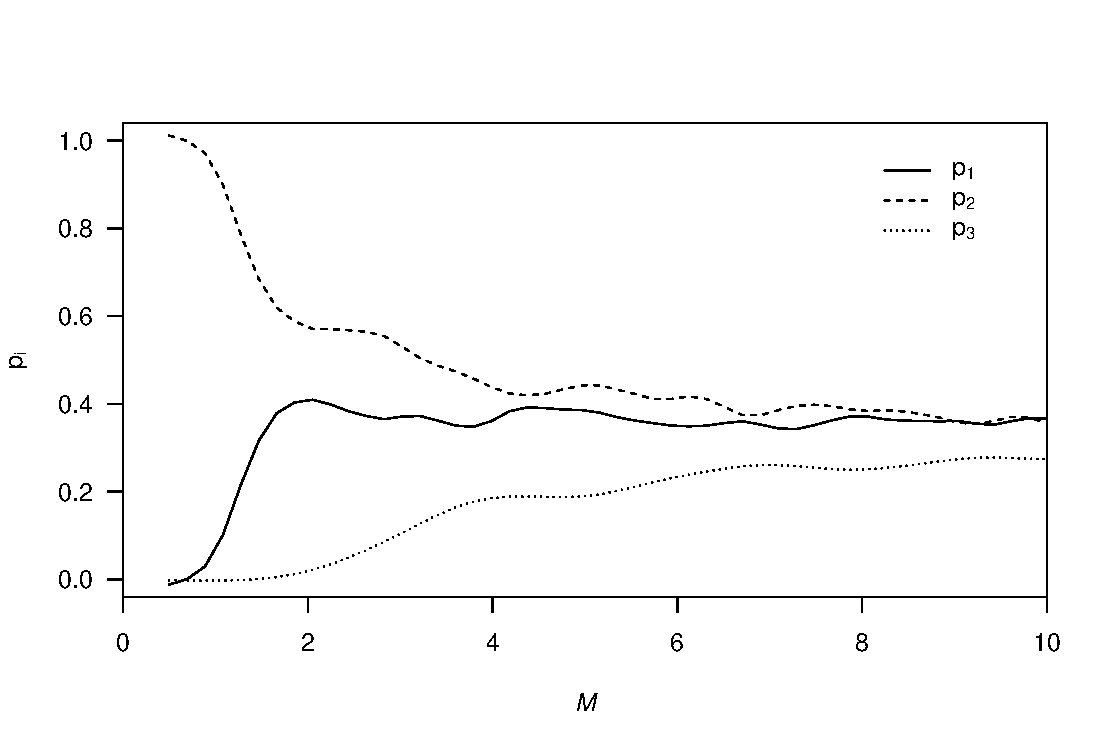
\includegraphics{voiConsAuc_files/figure-latex/evsi3simplot-1.pdf}
\caption{\label{fig:evsi3simplot}Simulation of optimal allocation of sampling among
three assets. Prior distributions of the three assets are as in figure
\ref{fig:evsi3heuplot}. Curves are smooth splines of the value of
\(p_i\) that maximizes the simulated EVSI for a given budget level of
\(M\). Note that the three curves are broadly similar to the heuristic
solution of figure \ref{fig:evsi3heuplot}.}
\end{figure}

\subsection*{Principles for allocating resources to
learning}\label{principles-for-allocating-resources-to-learning}
\addcontentsline{toc}{subsection}{Principles for allocating resources to
learning}

From the solutions to our simple model we can glean a number of rules of
thumb that agencies conducting conservation auctions should consider. By
examining the analytical solution to the two asset problem we can learn
a number of things, some of which hold when we increase the complexity
by adding a third asset and some of which do not. In examining both the
two-asset and three-asset solutions we have elucidated the following
principles guiding the allocation of learning resources in a
conservation auction.

\subsubsection*{Principle 1: Unequal sampling
allocation}\label{principle-1-unequal-sampling-allocation}
\addcontentsline{toc}{subsubsection}{Principle 1: Unequal sampling
allocation}

In general an optimized unequal allocation of sampling among the assets
in an auction will have greater EVSI and result in a more cost-effective
auction than simply allocating sampling equally among the assets.
However, the larger the budget for learning, the less having an optimal
allocation matters. For example, in the case study of figure
\ref{fig:evsi2anplot} we see that the peak of expected gain from
sampling optimally is for a small budget that is expected to return an
EVSI about half the EVPI. As the budget increases and with it EVSI
approaches EVPI asymptotically, the difference between an optimal
allocation of learning and a naive, even allocation becomes negligible.
When considering two assets, this principle only applies when the
uncertainty around each asset's cost-efficiency is unequal. Even if each
asset has a different expected cost-efficiency it is only optimal to
unevenly allocate learning if the variance of their prior
cost-efficiencies is unequal. However, when we consider a case with
three assets, then it is only optimal to allocate evenly when all the
prior means and all the prior variances are the same. That is to say, we
should only allocate learning equally when we are completely in the dark
about the rank order of asset cost efficiencies.

\subsubsection*{Principle 2: Learn first at the
margin}\label{principle-2-learn-first-at-the-margin}
\addcontentsline{toc}{subsubsection}{Principle 2: Learn first at the
margin}

Knowing that it is probably sub-optimal to allocate learning equally
among assets is only useful if one knows in what way they should
otherwise distribute sampling effort. Our second principle is that given
a small to moderate budget and some uncertainty about the
cost-efficiency of auction assets, it is wisest to allocate to assets on
the margin. By on the margin, we mean assets that are borderline cases
for potential investment. These are important cases for learning about
because new knowledge can impact whether those assets should be invested
in or not. By contrast, we can identify two other classes of asset:
those likely to be included among winning bids, and those unlikely to be
among the winners. For each of these classes, learning is less
preferential than the more marginal cases. In figure
\ref{fig:evsi3heuplot} this principle is illustrated by the fact that
assets 1 and 2 demand greater allocation of sampling than asset 3, as
asset 3 has the lowest prior mean cost-efficiency as well as the
greatest certainty. Further, for small budgets investment in learning
about asset 2 is preferred over asset 1.

\subsubsection*{Principle 3: Learn about the more uncertain
assets}\label{principle-3-learn-about-the-more-uncertain-assets}
\addcontentsline{toc}{subsubsection}{Principle 3: Learn about the more
uncertain assets}

Again, figure \ref{fig:evsi3heuplot} highlights the final principle.
Given the choice of allocating learning among assets with similar
cost-efficiency, it is more optimal to learn about the more uncertain.
This third principle however, interacts with the second, as it is only
more preferential to learn about asset 2 (the most uncertain
cost-efficiency) when the budget is small. But, when the budget is large
enough the allocation to learning about asset 1 approaches the
allocation to asset 2.

\subsection*{Conclusion}\label{conclusion}
\addcontentsline{toc}{subsection}{Conclusion}

This work begins to formalise a problem of information valuing for
conservation auctions. We have addressed this problem using a blend of
analytical, heuristic and simulation-based approaches, necessitated by
the absence of a closed-form solution for \(n>2\) assets. Clearly, this
work only scratches the surface of the value of learning in conservation
auctions. Yet the model, solutions and principles we outline above have
the potential to change the way information is used when implementing
conservation auctions. In the past information gathering to inform
conservation auctions has been either minimal, or when substantive,
allocated evenly across bids in the auction \citep[see
e.g.,][]{Miles2008}. Now, even if an auction conducting agency did not
wish to apply value of information formally, they may be able to apply
the principles we outline here to their pre-auction learning phase and
save learning resources, leading to more cost-effective auctions. This
could fundementally change the design of past conservation auctions,
such as Bush Tender \citep{Stoneham2003}, Bush Returns \citep{Miles2008}
and others \citep[e.g.,][]{Lobley1998, Hajkowicz2007, Hanley2014}, as it
demonstrates a benefit of emphasising learning in the period between
auction bids arriving, and the decision to invest in them. However, of
course some caveats apply. In our model we only consider cases where a
single asset is purchased at the end of the auction, and we assume that
uncertainty is normal distributed. Changing these assumptions may lead
to different results. Future work would help to verify and consolidate
the principles we outline above. Such work might include finding
analytical solutions for \(n > 2\) and even \(n > 3\), as well as
auctions with multiple successful bids and multiple auction rounds.

\bibliography{voiConsAuc.bib}

\newpage

\captionsetup{labelformat=empty}

\section*{\texorpdfstring{Appendix C: VOI for conservation auctions
heuristic solution \emph{n} =
2}{Appendix C: VOI for conservation auctions heuristic solution n = 2}}\label{appendix-c-voi-for-conservation-auctions-heuristic-solution-n-2}
\addcontentsline{toc}{section}{Appendix C: VOI for conservation auctions
heuristic solution \emph{n} = 2}

\textbf{Priors}

Let \(A_1\) and \(A_2\) be two assets. Each has some cost efficiency
\(c_1\) and \(c_2\), both of which are uncertain with prior probability
distributions,

\begin{equation}
c_1\sim\mathcal{N}(\mu_1, \sigma_1)
\label{eq:c1}
\end{equation}

and

\begin{equation}
c_2\sim\mathcal{N}(\mu_2, \sigma_2)
\label{eq:c2}
\end{equation}

where \(\mu_1\) and \(\mu_2\) are the prior means and \(\sigma_1\) and
\(\sigma_2\) are the prior standard deviations.

Let \(\pi=\Pr(c_1 > c_2)\) and therefore,

\begin{equation}
\pi = \Phi\left(\frac{\mu_1-\mu_2}{\sqrt{\sigma^2_1+\sigma^2_2}}\right)
\label{eq:c2}
\end{equation}

\textbf{Utilities}

If \(\pi > 1 - \pi\) then the optimal action is to purchase asset
\(A_1\), otherwise it is to purchase \(A_2\).

We can assign utilities to each combination of the condition of \(c_1\)
and \(c_2\), and each action such that,

\begin{equation}
\begin{aligned}
u(c_1 > c_2, A_1)&=1\\
u(c_1 < c_2, A_1)&=0\\
u(c_1 > c_2, A_2)&=0\\
u(c_1 < c_2, A_2)&=1\\
\end{aligned}
\label{eq:utilitiesapen}
\end{equation}

Therefore the expected values of taking each action are
\(\mathrm{E}[u(A_1)]=\pi\) and \(\mathrm{E}[u(A_2)]=1-\pi\).

\textbf{Value of perfect information}

If we could reduce the uncertainty in the prior probabilites of \(c_1\)
and \(c_2\) such that \(\pi\) approached either limit, then the expected
value of perfect information is,

\begin{equation}
\mathrm{EVPI}=1-\max(\pi, 1-\pi)=\min(\pi, 1-\pi)
\label{eq:evpiaucapen}
\end{equation}

\textbf{Preposterior analysis}

Now let's assume we can sample from some process and learn about \(c_1\)
and \(c_2\).\\
Let \(X_1\) and \(X_2\) be observations from a process described by the
following sampling distributions,

\begin{equation}
X_1\sim\mathcal{N}\left(c_1, 1\right)
\label{eq:x1}
\end{equation}

and

\begin{equation}
X_2\sim\mathcal{N}\left(c_2, 1\right)
\label{eq:x2}
\end{equation}

where for simplicity the standard deviation is one.

Furthermore, we can make \(Mp\) and \(M(p-1)\) observations of \(X_1\)
and \(X_2\) respectively. Where \(M\) is the total number of samples the
budget allows and \(p\) and \(p-1\) are proportions of that budget
allocated to each assets. Given the observations of \(X_1\) and \(X_1\)
with sample sizes \(Mp\) and \(M(p-1)\) we can update the prior beliefs
in \(c_1\) and \(c_2\) and arrive at posterior distributions,

\begin{equation} 
\begin{aligned}
c_1^\prime &\sim \mathcal{N}(\mu^\prime_1, \sigma^\prime_1)\\
c_2^\prime &\sim \mathcal{N}(\mu^\prime_2, \sigma^\prime_2)
\end{aligned}
\label{eq:posteriorcs}
\end{equation}

where,

\begin{equation}
\begin{aligned}
\mu^\prime_1 &= \frac{\mu_1 + X_1Mp\sigma^2_1}{Mp\sigma^2_1 + 1}\\
\sigma^\prime_1 &= \sqrt{\frac{\sigma^2_1}{Mp\sigma^2_1 + 1}}\\
\mu^\prime_2 &= \frac{\mu_2 + X_2M(p-1)\sigma^2_2}{M(p-1)\sigma^2_2 + 1}\\
\sigma^\prime_2 &= \sqrt{\frac{\sigma^2_2}{M(p-1)\sigma^2_2 + 1}}
\end{aligned}
\label{eq:posteriormusig}
\end{equation}

\textbf{Value of sample information}

Now we make the simplifying assumptions that
\(\mathrm{E}[X_1]=\mathrm{E}[c_1]=\mu_1\) and
\(\mathrm{E}[X_1]=\mathrm{E}[c_1]=\mu_1=0\).

In this scenario the prior probability of \(c_1>c_2\) is,

\begin{equation}
\pi=\Phi\left(\frac{\mu_1}{\sqrt{\sigma^2_1+\sigma^2_2}}\right)
\label{eq:priorpi}
\end{equation}

, and the posterior is

\begin{equation}
\pi^\prime=\Phi\left(\frac{\mu_1}{\sqrt{\frac{\sigma^2_1}{Mp\sigma^2_1 + 1}+\frac{\sigma^2_2}{M(p-1)\sigma^2_2 + 1}}}\right)
\label{eq:posteriorpi}
\end{equation}

We can now calculate the expected value of sample information,

\begin{equation}
\mathrm{EVSI}=\max(\pi^{\prime}, 1-\pi^{\prime})-\max(\pi, 1-\pi)
\label{eq:evsiaucapen}
\end{equation}

\textbf{Optimal sampling allocation}

With equations 10-12, for any given set of \(\mu_1\), \(\sigma_1\),
\(\mu_2\), and \(M\) we can find the optimal allocation to sample for
asset \(A_1\), \(p\) to maximise the value of sample information.

\textbf{Summary}

\begin{itemize}
\tightlist
\item
  Optimal allocation insensitive to ratio of \(\mu_a\) to \(\mu_b\).
\item
  Optimal allocation sensitive to ratio of \(\sigma_1\) to \(\sigma_2\).
\item
  Always preferential to sample asset with greater uncertainty.
\item
  Solution is symmetrical.
\item
  The \(M\) at which you start to allocate sampling to both assets is
  proportional to the ratio of \(\sigma_1\) to \(\sigma_2\).
\item
  The \(M\) at which you start to allocate sampling to both assets is
  insensitive to whether \(\sigma_1 < \sigma_2\) or
  \(\sigma_1 > \sigma_2\).
\item
  Optimal allocation always has greater EVSI when
  \(\sigma_1 \neq \sigma_2\).
\end{itemize}

\textbf{\(\mu_1 > \mu_2, \sigma_1 \gg \sigma_2\)}

First let's examine the case where our prior belief is that \(c_1\) is
somewhat greater than \(c_2\), where \(\mu_1=.2\) and \(\mu_2 = 0\) but
the uncertainty in \(\theta_1\) is far greater than in \(\theta_2\),
\(\sigma_1 = 2\) and \(\sigma_2 = .2\).

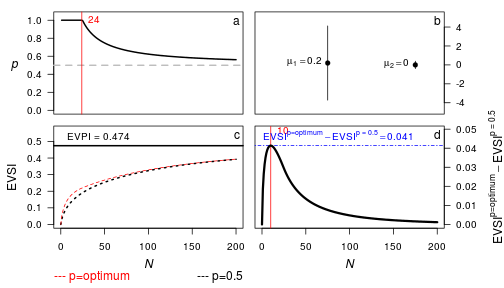
\includegraphics{figure/unnamed-chunk-2-1.png} \clearpage

In this case, until we can take more than a total of 24 samples
(\(N=24\)) the optimal allocation is to allocate all sampling effort to
asset \(A_1\) (a). With a total budget greater than 24 samples, we start
allocating sampling to asset \(A_2\) at a diminishing rate with total
sample size and asymptoting at \(p=0.5\). The expected value of sample
information (EVSI) increases with sample size with diminishing returns
asymptoting below the EVPI (c). At all sample sizes, the optimal
allocation has greater expected value than naive assumption of constant
allocation of \(p=0.5\). The greatest benefit of allocating optimally is
when the sample size is \(N=10\). As sample size increases the
additional benefit of allocating optimally declines asymptotically as
the optimal allocation approaches \(p=0.5\) (d).

\textbf{\(\mu_1 \simeq \mu_2, \sigma_1 \gg \sigma_2\)}

Holding all the other parameters constant, let's examine a scenario
where the prior expection of \(c_1\) is only marginally better than
\(c_2\) (i.e., reduce \(\mu_1\) to \(.01\)).

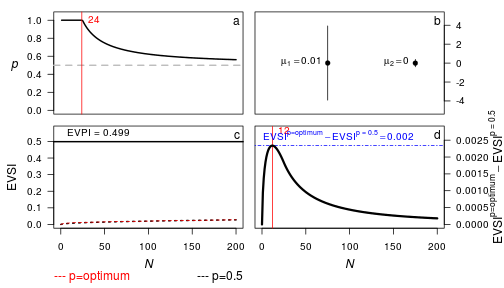
\includegraphics{figure/unnamed-chunk-3-1.png} \clearpage

We still allocate in the same way as before (a). The EVPI approaches its
theoretical maxmimum of 0.5. But the value of sample information
achievable for anything less than 200 samples is reduced to near zero
(c). The shape of the additional benefit from optimal allocation is the
same but the scale has reduced and the optimal value of N has increased
meaning more samples must be taken to maxmise the additional gain in
EVSI by using the optimal allocation vs the naive allocation of
\(p=0.5\) (d).

\textbf{\(\mu_1 \gg \mu_2, \sigma_1 \gg \sigma_2\)}

All other parameters still the same, but now with \(\mu_1=1\) much
greater than \(\mu_2\).

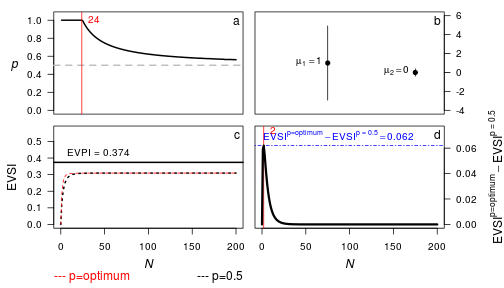
\includegraphics{figure/unnamed-chunk-4-1.png} \clearpage

Still same optimal allocation (a). EVPI reduced as we start already more
certain that \(A_1\) is a better asset than \(A_2\). The return on
investing in each additional sample diminishes quicker and sooner as
EVSI asymptotes at nearer EVPI (c). The additional benefit in EVSI seen
by sampling optimally has increased by peaks earlier at \(N=2\) (d).

\textbf{\(\mu_1 > \mu_2, \sigma_1 > \sigma_2\)}

Resetting \(\mu_1\) now we examine what happens when \(\sigma_1\) is
double \(\sigma_2\).

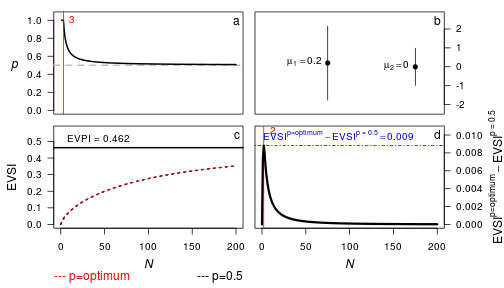
\includegraphics{figure/unnamed-chunk-5-1.png} \clearpage

The optimal allocation has the same shape as before but now we allocate
sampling to asset \(A_2\) sooner than before. Now if we take more than 3
samples we will allocate an increasing amount of them to asset \(A_2\)
(a). The EVPI has been reduced as we have started off more certain that
\(A_1\) is greater \(A_2\) (c). There is less advantage to sampling
optimally rather than the naive allocation but the point at which the
additional benefit in EVSI peaks is at higher \(N\) (\(N=2\)) than when
\(\sigma_1\) was much more than \(\sigma_2\) (d).

\textbf{\(\mu_1 > \mu_2, \sigma_1 = \sigma_2\)}

Now increase the precision of \(c_1\) so that \(\sigma_1 = \sigma_2\).

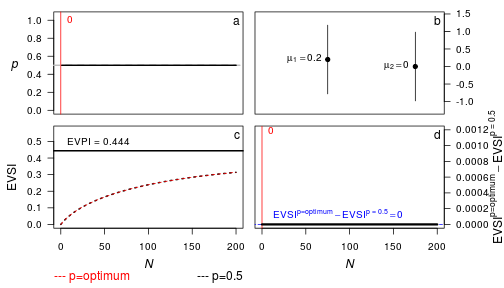
\includegraphics{figure/unnamed-chunk-6-1.png} \clearpage

Now the optimal allocation is to just allocate evenly between the assets
(i.e., the naive allocation is now optimal and there is effectively no
advantage to optimize) (a). The allocation is still insentive to the
value of \(\mu_1\) and the value of \(\sigma\)'s. Decreasing the prior
precisions increases EVPI, and with it the point at which EVSI vs \(N\)
asymptotes, but without changing the rate EVPI increases with \(N\).
Increaseing the value of \(\mu_1\) decreases EVPI (but less sensitively
than changing the precision) and also increases the rate at which EVPI
vs \(N\) approaches EVPI (c).

\textbf{\(\mu_1 > \mu_2, \sigma_1 \ll \sigma_2\)}

Returning to the original paramterisation now reverse the prior
precisions so that \(\tau^\prime_a\) is much greater than
\(\tau^\prime_b\).

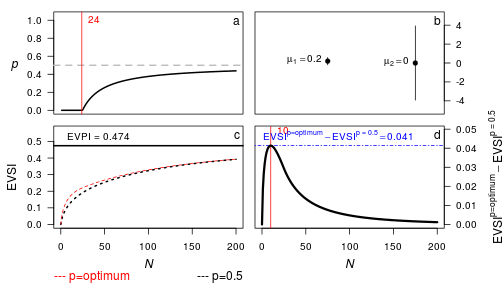
\includegraphics{figure/unnamed-chunk-7-1.png} \clearpage

The allocation is the same but now reflected so that we still allocate
to the asset with more uncertainty (a). This applies no matter what the
other parameter values are (i.e., the problem is symetrical).

\captionsetup{labelformat=default}

\newpage

\captionsetup{labelformat=empty}

\section*{\texorpdfstring{Appendix D: VOI for conservation auctions
heuristic solution \emph{n} =
3}{Appendix D: VOI for conservation auctions heuristic solution n = 3}}\label{appendix-d-voi-for-conservation-auctions-heuristic-solution-n-3}
\addcontentsline{toc}{section}{Appendix D: VOI for conservation auctions
heuristic solution \emph{n} = 3}

\textbf{Priors}

Let \(A_1\), \(A_2\), \(A_3\) be assets. Each has some value \(c_1\),
\(c_2\), and \(c_3\) which are uncertain with a joint prior probability
distribution,

\begin{equation}
\begin{bmatrix}c_1 \\ c_2 \\ c_3\end{bmatrix}\sim\mathcal{N}\left(\begin{bmatrix}\mu_1 \\ \mu_2 \\ \mu_3\end{bmatrix}, \begin{bmatrix}\sigma^2_1 & 0 & 0 \\ 0 & \sigma^2_2 & 0\\ 0 & 0 & \sigma^2_3 \end{bmatrix}\right)
\label{eq:jointprior}
\end{equation}

where \(\mu_1\), \(\mu_2\), and \(\mu_3\) are means and \(\sigma_1\),
\(\sigma_2\) and \(\sigma_3\) are the prior standard deviations.

\textbf{Utilities}

We assign utilities to each rank order of \(c_1\), \(c_2\), and \(c_3\)
in combination with each action of purchasing one of \(A\), \(B\) or
\(C\),

\begin{equation}
\begin{aligned}
u(A_1, c_1 > c_2 > c_3)&=1\\
u(A_1, c_1 > c_3 > c_2)&=1\\
u(A_1, c_2 > c_1 > c_3)&=0.5\\
u(A_1, c_3 > c_1 > c_2)&=0.5\\
u(A_1, c_2 > c_3 > c_1)&=0\\
u(A_1, c_3 > c_2 > c_1)&=0\\
u(A_2, c_2 > c_1 > c_3)&=1\\
\mathrm{etc...}&
\end{aligned}
\label{eq:utilitiesapen2}
\end{equation}

such that utility is maximised when we purchase the highest ranked
asset, zero when we purchase the lowest ranked and somewhere inbetween
when we purchase the middle ranked asset.

\textbf{Ranking probabilties}

We can express the probability of any assets being in a given rank order
as the probabililty of two differences being less than zero. Such that,
for example,

\begin{equation}
\Pr(c_1 > c_2 > c_3) = \Pr(c_2 - c_1 < 0,  c_3 - c_2 < 0)
\label{eq:probrankapen}
\end{equation}

Given this we define two new variables, \(z_1\) and \(z_2\) where

\begin{equation}
\begin{aligned}
  z_1 &= c_2 - c_1,\\
  z_2 &= c_3 - c_2
\end{aligned}
\label{eq:z12apen}
\end{equation}

Even if \(c_1\), \(c_2\), and \(c_3\) are all uncorrelated \(z_1\) and
\(z_2\) will not be, where

\begin{equation}
\mathrm{cov}(z_1, z_2)=\mathrm{cov}(c_1, c_2) - \mathrm{var}(c_2) - \mathrm{cov}(c_1, c_3) + \mathrm{cov}(c_2, c_3)
\label{eq:covz}
\end{equation}

Which, when \(c_1\), \(c_2\), and \(c_3\) are all uncorrelated
simplifies to

\begin{equation}
\mathrm{cov}(z_1, z_2)=-\mathrm{var}(c_2)
\label{eq:covz2}
\end{equation}

Therefore the joint distribution of \(z_1\) and \(z_2\) is,

\begin{equation}
\begin{bmatrix}z_1\\z_2\end{bmatrix}
  \sim\mathrm{N}\left(
  \begin{bmatrix}\mu_2-\mu_1\\\mu_3-\mu_2\end{bmatrix},
  \begin{bmatrix}\sigma^2_1+\sigma^2_2&-\sigma^2_2\\-\sigma^2_2&\sigma^2_2+\sigma^2_3\end{bmatrix}\right)
\label{eq:jointzapen}
\end{equation}

To obtain \(\Pr(c_1 > c_2 > c_3)\) we evalute the multivariate
cumulative distribution function of \(z_1\) and \(z_2\),

\begin{equation}
\Phi(z_1,z_2)
\label{eq:phiz}
\end{equation}

within the limits, \(-\infty\) and 0.

\textbf{Expected value of perfect information}

To calculate the prior expected utility of purchasing any asset, we
weight the utilities for that action (eqn. 2) by the relevant
probablities calculated from eqns. 3--9. For instance;

\begin{equation}
\begin{aligned}
  \mathrm{E}[u(A_1)] = & 1 \times \Pr(c_1 > c_2 > c_3) + 1 \times \Pr(c_1 > c_3 > c_2)\,+ \\
  &0.5 \times \Pr(c_2 > c_1 > c_3) + 0.5 \times \Pr(c_3 > c_1 > c_2)\,+ \\
  &0 \times \Pr(c_2 > c_3 > c_1) + 0 \times \Pr(c_3 > c_2 > c_1)
\end{aligned}
\label{eq:EuA1apen}
\end{equation}

The expected value of perfect information then is,

\begin{equation}
\mathrm{EVPI}=1-\max(\mathrm{E}[u(A_1)],\mathrm{E}[u(A_2)],\mathrm{E}[u(A_3)])
\label{eq:evpiapen2}
\end{equation}

\textbf{Updating}

Now suppose we can update the priors for \(c_1\), \(c_2\), and \(c_3\)
by taking \(M\) samples from sampling distrubutions with, for
simplicity, some fixed variance of 1 and centered on \(\mu_1\),
\(\mu_2\) and \(\mu_3\) respectively. Further, we can define \(p_1\) and
\(p_2\) as the proportion of the \(M\) samples allocated to sampling for
\(A_1\) and \(A_2\) respectively with \(1 - p_1 - p_2\) being allocated
to \(A_3\). We can then use these samples to update the priors for
\(c_1\), \(c_2\), and \(c_3\) to obtain preposterior estimates,
\(c^\prime_1\), \(c^\prime_2\), and \(c^\prime_3\), where,

\begin{equation}
\begin{bmatrix}c^\prime_1 \\ c^\prime_2 \\ c^\prime_3\end{bmatrix}\sim\mathcal{N}\left(\begin{bmatrix}\mu_1 \\ \mu_2 \\ \mu_3\end{bmatrix}, \begin{bmatrix}\frac{\sigma^2_1}{Mp_1\sigma^2_1 + 1} & 0 & 0 \\ 0 & \frac{\sigma^2_2}{Mp_2\sigma^2_2 + 1} & 0\\ 0 & 0 & \frac{\sigma^2_3}{M(1 - p_1 - p_2)\sigma^2_3 + 1} \end{bmatrix}\right)
\label{eq:jointpost}
\end{equation}

\textbf{Expected value of sample information}

For any given new rank order, based on the updated preposterior
distributions, we can again calculate a probablity by defining new
variables (i.e., \(z^\prime_1\) and \(z^\prime_2\)) and evalute their
multivariate cumulative distribution as in eqns. 3--9. Therefore we can
obtain the preposterior expected utilities for each purchase action by
weighting the preposterior probablites by their respective utilities as
in eqn. 10. Accordingly the expected vale of sample information is

\begin{equation}
\mathrm{EVSI}=\max(\mathrm{E}^\prime[u(A_1)],\mathrm{E}^\prime[u(A_2)],\mathrm{E}^\prime[u(A_3)])-\max(\mathrm{E}[u(A_1)],\mathrm{E}[u(A_2)],\mathrm{E}[u(A_3)])
\label{eq:evsiapen2}
\end{equation}

\textbf{Optimisation}

Using eqns 8-13 we can find the optimal values of \(p_1\) and \(p_2\)
for any given \(M\) that will maximise the EVSI. Below we examine a
number of \_\_Case studies for different sets of prior distrbutions for
\(c_1\), \(c_2\) and \(c_3\).

\textbf{Summary}

\begin{itemize}
\tightlist
\item
  Optimal allocation sensitive to ratios of \(\mu\)'s.
\item
  Optimal allocation sensitive to ratio of \(\sigma\)'s.
\item
  Not always preferential to sample asset with greater uncertainty.
\item
  Solution is symmetrical.
\end{itemize}

\textbf{Case study 1: homogenous prior \(\sigma\)'s and homogenous prior
means}

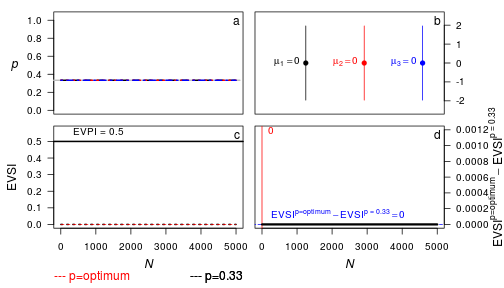
\includegraphics{figure/x000_1_1_1-1.png} \clearpage

\textbf{Case study 2a: homogenous prior \(\sigma\)'s and heterogenous
prior means}

\(\mu_1 = \mu_2 > \mu_3\)

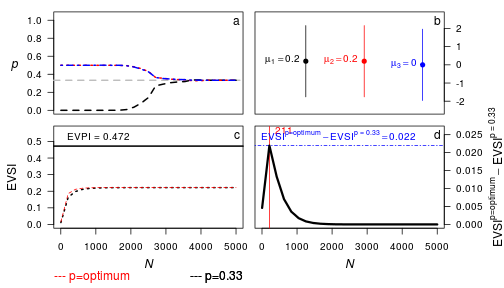
\includegraphics{figure/x110_1_1_1c-1.png} \clearpage

\textbf{Case study 2b: homogenous prior \(\sigma\)'s and heterogenous
prior means}

\(\mu_1 > \mu_2 = \mu_3\)

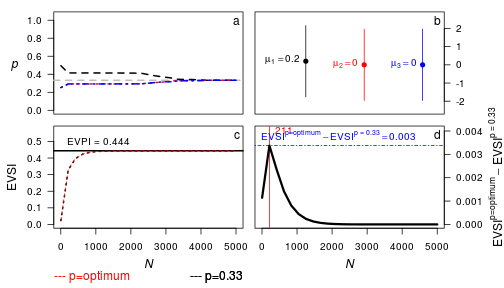
\includegraphics{figure/x100_1_1_1c-1.png} \clearpage

\textbf{Case study 2c: homogenous prior \(\sigma\)'s and heterogenous
prior means}

\(\mu_1 > \mu_2 > \mu_3\)

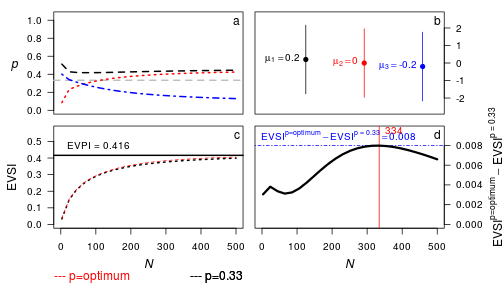
\includegraphics{figure/x10n1_1_1_1c-1.png} \clearpage

\textbf{Case study 3a: heterogenous prior \(\sigma\)'s and heterogenous
prior means}

\(\mu_1 > \mu_2 = \mu_3\)

\(\sigma_1 > \sigma_2 = \sigma_3\)

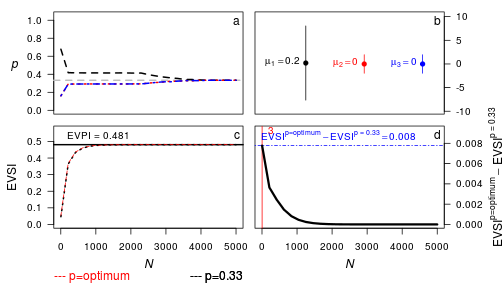
\includegraphics{figure/x100___1_1_1c-1.png} \clearpage

\textbf{Case study 3b: heterogenous prior \(\sigma\)'s and heterogenous
prior means}

\(\mu_1 > \mu_2 = \mu_3\)

\(\sigma_1 < \sigma_2 = \sigma_3\)

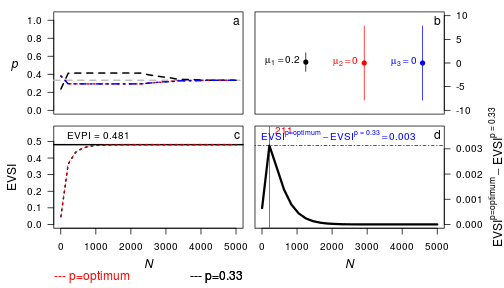
\includegraphics{figure/x1001_1_1c-1.png} \clearpage

\textbf{Case study 3c: heterogenous prior \(\sigma\)'s and heterogenous
prior means}

\(\mu_1 = \mu_2 > \mu_3\)

\(\sigma_1 = \sigma_2 < \sigma_3\)

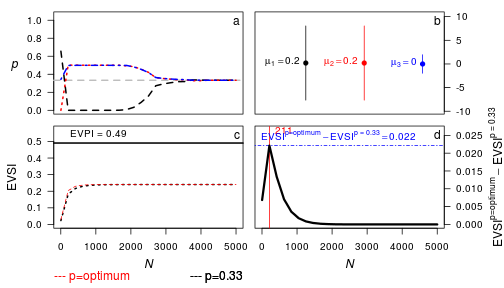
\includegraphics{figure/x110__1__1_1c-1.png} \clearpage

\textbf{Case study 3d: heterogenous prior \(\sigma\)'s and heterogenous
prior means}

\(\mu_1 > \mu_2 = \mu_3\)

\(\sigma_1 = \sigma_2 > \sigma_3\)

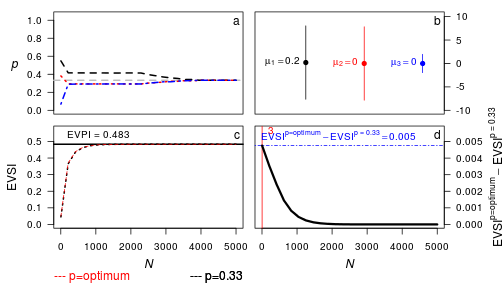
\includegraphics{figure/x100__1__1_1c-1.png} \clearpage

\textbf{Case study 3e: heterogenous prior \(\sigma\)'s and heterogenous
prior means}

\(\mu_1 > \mu_2 = \mu_3\)

\(\sigma_1 = \sigma_2 < \sigma_3\)

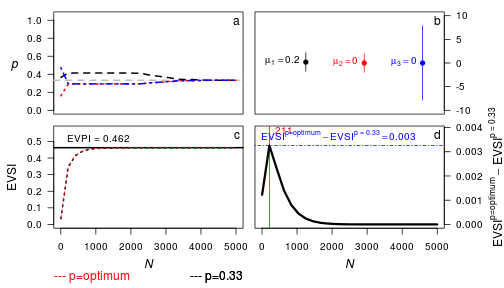
\includegraphics{figure/x100_1_1__1c-1.png} \clearpage

\textbf{Case study 3f: heterogenous prior \(\sigma\)'s and heterogenous
prior means}

\(\mu_1 = \mu_2 > \mu_3\)

\(\sigma_1 = \sigma_3 > \sigma_2\)

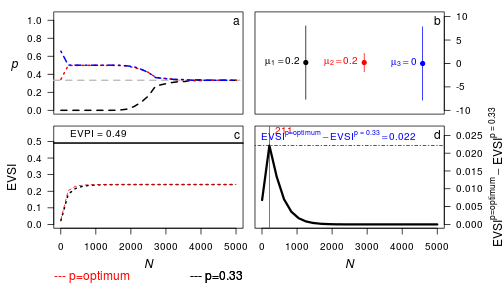
\includegraphics{figure/x110__1_1__1c-1.png} \clearpage

\textbf{Case study 3g: heterogenous prior \(\sigma\)'s and heterogenous
prior means}

\(\mu_1 = \mu_2 > \mu_3\)

\(\sigma_1 = \sigma_3 < \sigma_2\)

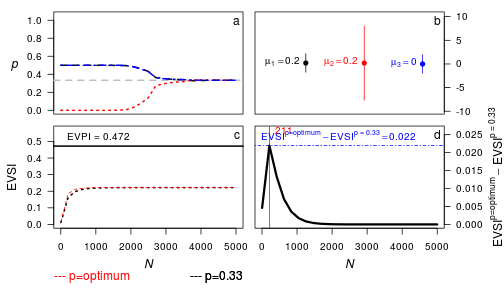
\includegraphics{figure/x110_1__1_1c-1.png} \clearpage

\textbf{Case study 3h: heterogenous prior \(\sigma\)'s and heterogenous
prior means}

\(\mu_1 > \mu_2 = \mu_3\)

\(\sigma_1 < \sigma_2 < \sigma_3\)

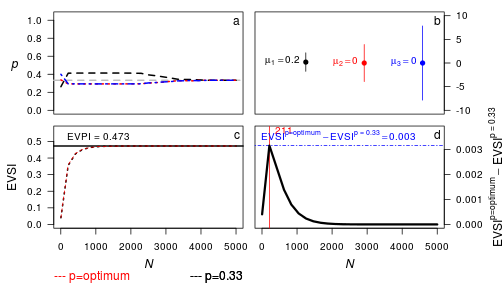
\includegraphics{figure/x100_1__1___1c-1.png} \clearpage  

\textbf{Case study 3i: heterogenous prior \(\sigma\)'s and heterogenous
prior means}

\(\mu_1 > \mu_2 = \mu_3\)

\(\sigma_2 < \sigma_1 < \sigma_3\)

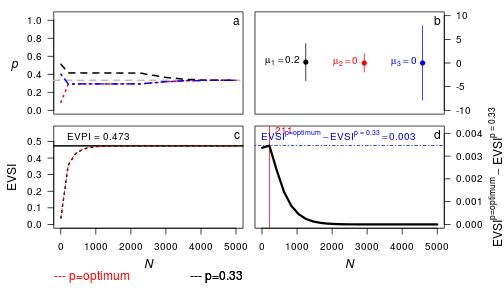
\includegraphics{figure/x100__1_1___1c-1.png} \clearpage

\textbf{Case study 3j: heterogenous prior \(\sigma\)'s and heterogenous
prior means}

\(\mu_1 > \mu_2 = \mu_3\)

\(\sigma_1 > \sigma_2 > \sigma_3\)

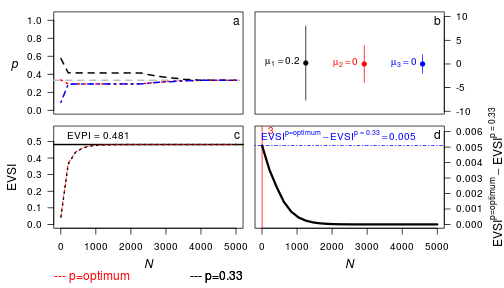
\includegraphics{figure/x100___1__1_1c-1.png} \clearpage

\textbf{Case study 3k: heterogenous prior \(\sigma\)'s and heterogenous
prior means}

\(\mu_1 = \mu_2 > \mu_3\)

\(\sigma_1 < \sigma_2 < \sigma_3\)

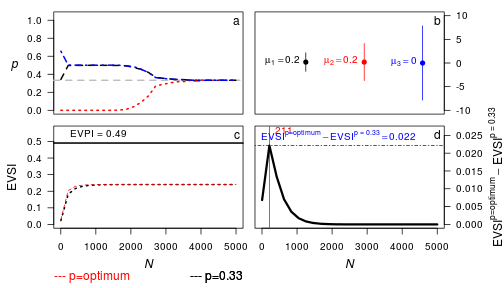
\includegraphics{figure/x110_1__1___1c-1.png} \clearpage

\textbf{Case study 3l: heterogenous prior \(\sigma\)'s and heterogenous
prior means}

\(\mu_1 = \mu_2 > \mu_3\)

\(\sigma_1 < \sigma_3 < \sigma_2\)

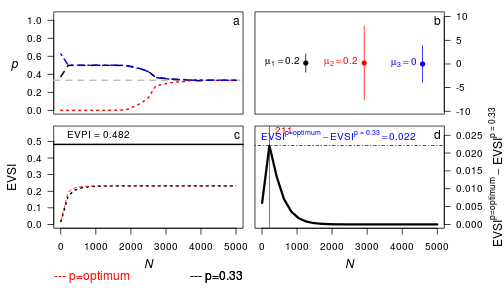
\includegraphics{figure/x110_1___1__1c-1.png} \clearpage  

\textbf{Case study 3m: heterogenous prior \(\sigma\)'s and heterogenous
prior means}

\(\mu_1 = \mu_2 > \mu_3\)

\(\sigma_1 > \sigma_2 > \sigma_3\)

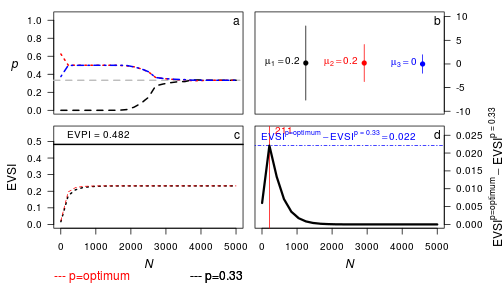
\includegraphics{figure/x110___1__1_1c-1.png} \clearpage

\textbf{Case study 3n: heterogenous prior \(\sigma\)'s and heterogenous
prior means}

\(\mu_1 > \mu_2 > \mu_3\)

\(\sigma_1 < \sigma_2 = \sigma_3\)

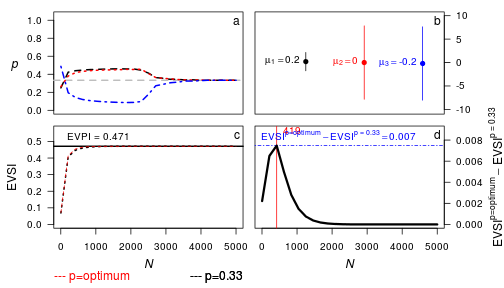
\includegraphics{figure/x10n1_1__1__1c-1.png} \clearpage

\textbf{Case study 3o: heterogenous prior \(\sigma\)'s and heterogenous
prior means}

\(\mu_1 > \mu_2 > \mu_3\)

\(\sigma_1 = \sigma_2 < \sigma_3\)

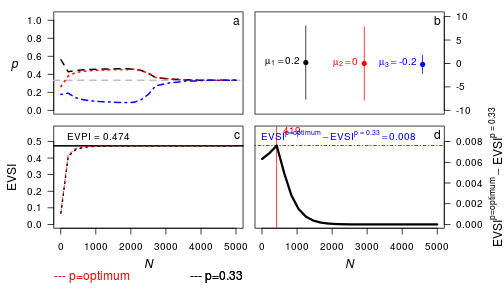
\includegraphics{figure/x10n1__1__1_1c-1.png} \clearpage

\textbf{Case study 3p: heterogenous prior \(\sigma\)'s and heterogenous
prior means}

\(\mu_1 > \mu_2 > \mu_3\)

\(\sigma_1 = \sigma_3 > \sigma_2\)

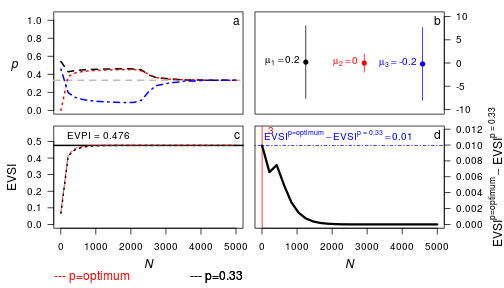
\includegraphics{figure/x10n1__1_1__1c-1.png} \clearpage  

\textbf{Case study 3q: heterogenous prior \(\sigma\)'s and heterogenous
prior means}

\(\mu_1 > \mu_2 > \mu_3\)

\(\sigma_1 = \sigma_2 < \sigma_3\)

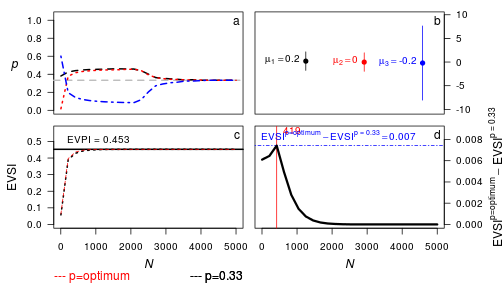
\includegraphics{figure/x10n1_1_1__1c-1.png} \clearpage

\textbf{Case study 3r: heterogenous prior \(\sigma\)'s and heterogenous
prior means}

\(\mu_1 > \mu_2 > \mu_3\)

\(\sigma_1 > \sigma_2 = \sigma_3\)

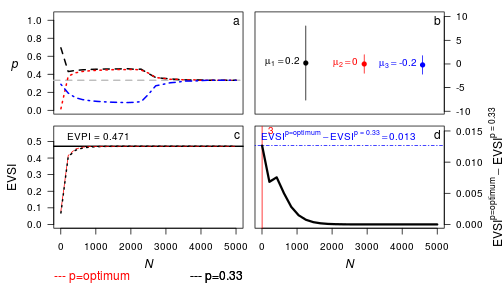
\includegraphics{figure/x10n1__1_1_1c-1.png} \clearpage

\textbf{Case study 3s: heterogenous prior \(\sigma\)'s and heterogenous
prior means}

\(\mu_1 > \mu_2 > \mu_3\)

\(\sigma_1 = \sigma_3 < \sigma_2\)

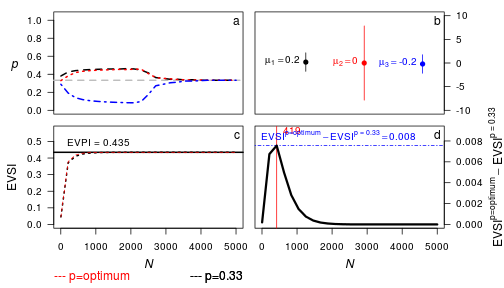
\includegraphics{figure/x10n1_1__1_1c-1.png} \clearpage

\textbf{Case study 3t: heterogenous prior \(\sigma\)'s and heterogenous
prior means}

\(\mu_1 > \mu_2 > \mu_3\)

\(\sigma_1 < \sigma_2 < \sigma_3\)

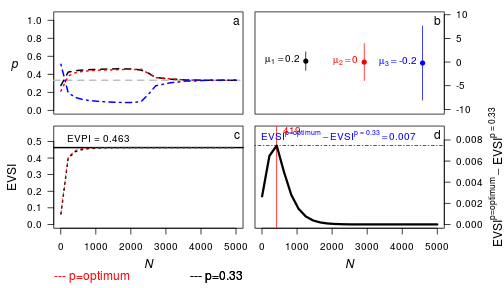
\includegraphics{figure/x10n1_1__1___1c-1.png} \clearpage  

\textbf{Case study 3u: heterogenous prior \(\sigma\)'s and heterogenous
prior means}

\(\mu_1 > \mu_2 > \mu_3\)

\(\sigma_2 < \sigma_1 < \sigma_3\)

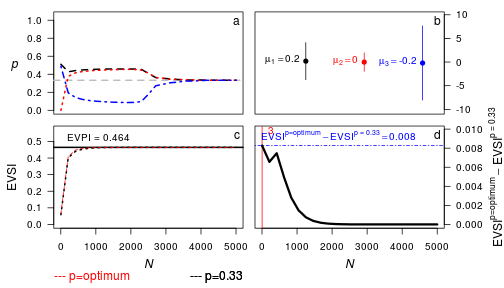
\includegraphics{figure/x10n1__1_1___1c-1.png} \clearpage

\textbf{Case study 3v: heterogenous prior \(\sigma\)'s and heterogenous
prior means}

\(\mu_1 > \mu_2 > \mu_3\)

\(\sigma_1 < \sigma_3 < \sigma_2\)

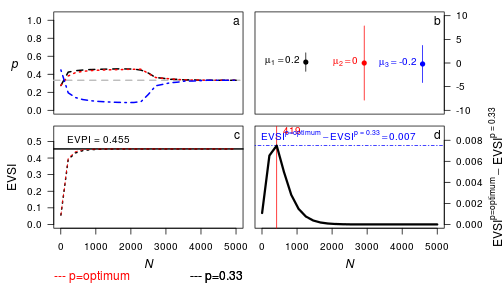
\includegraphics{figure/x10n1_1___1__1c-1.png} \clearpage

\textbf{Case study 3w: heterogenous prior \(\sigma\)'s and heterogenous
prior means}

\(\mu_1 > \mu_2 > \mu_3\)

\(\sigma_1 > \sigma_3 > \sigma_2\)

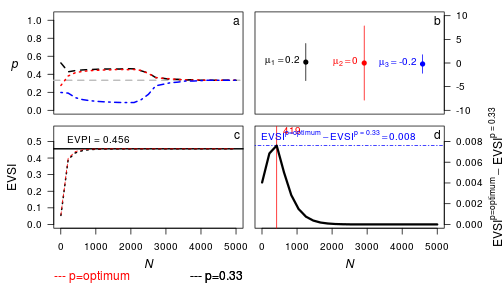
\includegraphics{figure/x10n1__1___1_1c-1.png} \clearpage

\textbf{Case study 3x: heterogenous prior \(\sigma\)'s and heterogenous
prior means}

\(\mu_1 > \mu_2 > \mu_3\)

\(\sigma_1 > \sigma_2 > \sigma_3\)

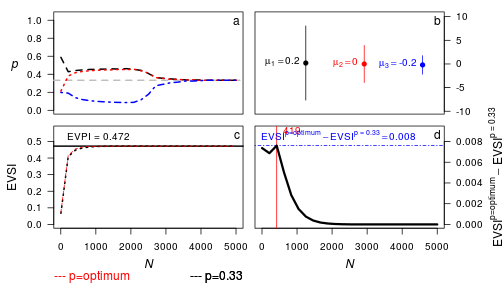
\includegraphics{figure/x10n1___1__1_1c-1.png} \clearpage

\captionsetup{labelformat=default}


\end{document}
